\documentclass[a4paper]{article}
\usepackage[utf8x]{inputenc}
\usepackage[english]{babel}
\usepackage{a4wide}
\usepackage[pdftex,hidelinks]{hyperref}
\usepackage{float}
\usepackage{graphicx}
\usepackage{booktabs}
\usepackage{fancyhdr}
\usepackage{lastpage}

\pagestyle{fancy}
\fancyhf{}

\rfoot{Page \thepage~of~\pageref{LastPage}}
\newcommand{\centered}[1]{\begin{tabular}{l} #1 \end{tabular}}

\begin{document}

\title{????????PROJECT NAME????????}
%todo: Member pictures
\author{%
    \begin{tabular}{lll}
        \centered{95145} & \centered{Eva Verboom} &
        \centered{
\includegraphics[width=3cm]{images/eva.jpeg}} \\
        \centered{95383} & \centered{Felipe Gorostiaga} &
        \centered{
\includegraphics[width=3cm]{images/felipe.jpg}} \\
        \centered{97144} & \centered{Pedro Mendes} &
        \centered{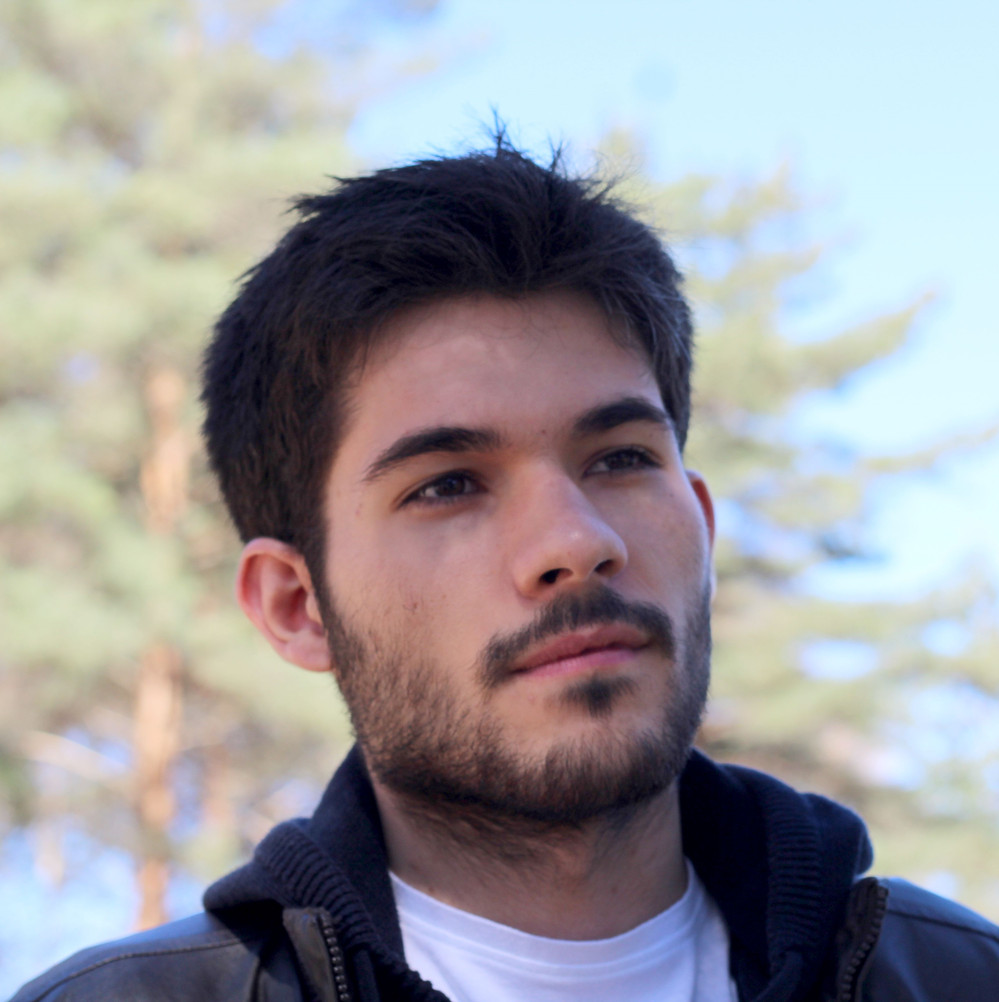
\includegraphics[width=3cm]{images/pedro.jpg}} \\
    \end{tabular}
}

\date{\today}

\begin{titlepage}

    %título
    \begin{center}
        \begin{minipage}{0.75\linewidth}
            \centering
            \vspace{1.5cm}
            %títulos
            \href{https://fenix.tecnico.ulisboa.pt/disciplinas/SIRS7/2019-2020/1-semestre}
            {\scshape\LARGE Network and Computer Security} \par
            \vspace{1cm}
            {\scshape\Large Alameda} \par
            \vspace{1cm}
            {\scshape\Large Group 28} \par
            \vspace{1.5cm}

            \maketitle
        \end{minipage}
    \end{center}

\end{titlepage}

\tableofcontents

\pagebreak

%% I  Problem (Given the chosen scenario, where is security necessary? What is the main problem
%% being solved? Use around 200 words)
\section{The Problem}

During this project we will be working on the development of a secure child locator. As a parent,
one might want to track their children to ensure that they aren't straying too far from where they
are supposed to be and in case something is wrong, to find them. Of course, this is very sensitive
information, because you do not want malicious actors to be able to track your children and misuse
the information in any way. Therefore, accessing the information should only be possible for
authorised guardian and secure communication of the child's location is required as well as secure
storage on remote servers. We will tackle the security issues in the same order, first we will
ensure that the application only allows authorised users to access the information they are allowed
to access and then we will work on secure communication protocols. When this is ensured, we will
direct our focus on the servers where the data is stored, assuming that the server is
``honest-but-curious''.

%% a. Requirements (Which security requirements were identified for the solution? Present as a list)
\subsection{Requirements}

The security requirements needed to solve this problem are then:
\begin{itemize}
    \item The system must maintain the confidentially of all data that is classified as confidential;
    \item The system must identify users in a reliable way;
    \item The system must only show data to users if they are authorised to access that particular data;
    \item The system must not allow anyone to change localisation data;
    \item
\end{itemize}

%% b. Trust assumptions (Be explicit about trust relationships. Who will be fully trusted,
%% partially trusted, or untrusted)
\subsection{Trust Assumptions}
There are three groups of actors to be distinguished here: the children, the guardians and the external servers. Both children and guardians shall be fully trusted by the system (though only after authentication) and the external servers shall be partially trusted. All other actors that can in some way have access to the data are untrusted parties.

%% Proposed solution (overview with diagram and explanation with around 200 words or less)
\section{Proposed Solution}

%% a) Deployment (describe distinct machines and how they will be interconnected)
\subsection{Deployment}

The system will consist of 3 moving parts:

\begin{itemize}
    \item A centralised server (may or may not be a distributed system)
    \item Multiple parent clients
    \item Multiple child clients
\end{itemize}

To achieve secure communication from the child and parent clients both will require appropriate methods
of authentication.

\subsubsection{Parent Client}
The parent will have to establish a public and private key pair with the server to ensure confidentiality
and a local only password to use the app (maybe also making use of fingerprint scanning).

\subsubsection{Child Client}
The child and parent clients need to agree on a private key that only they know, to encrypt every piece of
data they send to the server. Afterwords the child client also establishes as secure channel with the server.

%% Secure channel(s) to configure (identify communication entities; existing library/tool to use;
%% what keys will exist and how will they be distributed)
\subsection{Secure channels}
Effectively the entities that will interact in the system are only the child and parent clients,
the server will only serve remote storage for the data. By using private key encryption for the data
we ensure confidentiality and integrity of the data and by using public private key pairs for communication
with the server we ensure authenticity.

%% Secure protocol(s) to develop (identify communication entities; language to use for
%% implementation; what keys will exist and how will they be distributed)
\subsection{Secure Protocols}


\section{Plan}

%% Versions (Describe basic, intermediate and advanced versions of the work and when are they
%% expected to be achieved)
\subsection{Project Versions}


\subsubsection{Minimum Viable Product (MVP)}
The MVP of our product should consist of the following:
\begin{itemize}
    \item Parent accounts which can be authenticated by the server;
    \item Parents should be able to create accounts for their children;
    \item Child clients should be able to localise themselves outdoors;
    \item A central server that communicates with all clients and authorises guardians to view the tracking data of their children;
    \item Secure channels for data communication between the server and all clients.
\end{itemize}

\subsubsection{Intermediate}

\begin{itemize}
    \item Child clients should also be able to locate themselves indoors;
    \item Child clients should be able to send alerts, when they press an SOS button or go out of safe zones;
    \item Parent clients should be able to receive alerts;
    \item Data should be send encrypted, such that only guardians are able to track the child and the server is unable to know the location.
\end{itemize}


\subsubsection{Full Feature Release}


\begin{itemize}
    \item Login as a user should be done using two-factor authentication;
    \item
\end{itemize}

%% Effort commitments (table containing one row per week until the submission date; and one
%% column per group member with expected activities for the given week; some cells may be left
%% blank because of work in other courses)
\subsection{Effort Commitments}

\begin{tabular}{llll}
    \toprule
    Week & Eva & Felipe & Pedro\\ \toprule
    28 Oct --- 3 Nov & x & x & x\\\midrule
    4 Nov --- 10 Nov & x & x & x\\\midrule
    11 Nov --- 17 Nov & x & x & x\\\midrule
    18 Nov --- 24 Nov & x & x & x\\\midrule
    25 Nov --- 1 Dec & x & x & x\\\midrule
    2 Dec --- 8 Dec & x & x & x\\\midrule
    9 Dec --- 15 Dec & x & x & x\\\bottomrule
\end{tabular}

%% References (tools, libraries, etc. that will be used in the project. State if each tool has been
%% found/installed/tested at the time of proposal)
\section{References}
The main technology for developing the applications will be the android studio and the built in Java
encryption libraries (which have been tested at the time of writing this proposal).

For the server we intend to use postgress

\end{document}
